% vim:encoding=utf8 ft=tex sts=2 sw=2 et:

\documentclass{classrep}
\usepackage[utf8]{inputenc}

\usepackage{listings}
\usepackage{graphicx}
\studycycle{Informatyka, studia niestacjonarne}
\coursesemester{IV}

%\coursename{Angelologia teoretyczna i stosowana}
\coursename{Inteligentna Analiza Danych}
\courseyear{2017/2018}

\courseteacher{mgr Rogalski}
\coursegroup{sobota, 10:45}

\author{
  \studentinfo{Marcin Pajkowski}{211968} \and
  \studentinfo{Rafał Warda}{214067}
}

\title{Zadanie 2a: Perceptron wielowarstwowy}

\begin{document}
\maketitle

\section{Wstęp}
Celem zadania było napisanie programu implementującego perceptron wielowarstwowy z wykorzystaniem wstecznej propagacji błędów jako mechanizmu nauki.

\section{Opis działania}
Zaimplementowany program pozwala na stworzenie sieci neuronowej o dowolnej ilości neuronów zorganizowanych w dowolną ilość warstw (oczywiście ograniczeniem jest platforma, na której skompilujemy i uruchomimy program). Parametry takie jak: momentum, współczynnik nauki, możliwość włączenia biasu możemy ustalić z poziomu linii poleceń.

Wagi neuronów obliczających są inicjalizowane wartościami pseudolosowymi z zakresu [-0.5, +0.5]. Wartości wag są aktualizowane co epokę, kolejne wzorce treningowe są podawane na wejście sieci w kolejności losowej.
\clearpage
\subsection{Propagacja sygnału}
Neurony warstwy wejściowej powielają wejście zadane przez użytkownika sieci neuronowej, a neurony warstwy wyjściowej i warstw ukrytych są neuronami o nieliniowej funkcji aktywacji. Nieliniowość jest odwzorowana funkcją sigmoidalną


$$ f_a(x) =  \frac{1}{{1} + e^{-x} } $$
mającą pochodną

$$ f_a'(x) = f(x)(1-f(x)) $$

Wyjście j-tego neuronu i-tej warstwy (gdzie warstwa jest warstwą ukrytą lub wyjściową) można wyznaczyć wyliczając najpierw sumę iloczynu jego wejść i wag

$$ suma_{ij} = \sum_{k=1}^{n} waga_k \cdot wejście_k $$

Następnie otrzymaną sumę przetwarzamy przy użyciu wyżej wymienionej funkcji aktywacyjnej

$$ wyjście_{ij} = f_a(suma_{ij}) $$

Reasumując: wejścia warstwy liniowej są przekazywane do każdego neuronu w kolejnej warstwie, a wyjścia każdego neuronu tej warstwy są mapowane jako wejścia neuronów kolejnych warstw. Wynik jest wyjściem ostatniej warstwy.

\subsection{Trening sieci}
\subsubsection{Podstawowe założenia}
Wyniki otrzymane na wyjściu sieci po przejściu jednokrotnie wyżej opisanego procesu wysoce prawdopodobnie nie spełnią oczekiwań użytkownika sieci. Aby sieć potrafiła zrealizować narzucone jej zadania, należy ją wytrenować. Stosowana jest w tym celu \textbf{wsteczna propagacja}.

Samo pojęcie treningu sieci można utożsamić z minimalizacją błędu średniokwadratowego.
$$ MSE = \frac{1}{2}((wzorzecwyjściowy_i-wyjście_i)^2 $$

Proces treningu powtarzany jest do momentu osiągnięcia satysfakcjonującego wyniku lub przez określoną liczbę iteracji. Każdą taką iterację nazywamy \textbf{epoką}.

W ciągu każdej epoki dokonywana jest wspomniana wyżej propagacja błędu oraz aktualizacja wag neuronów.
\clearpage
\subsubsection{O propagacji wstecznej}

Propagacja wsteczna jest algorytmem pozwalającym skutecznie zniwelować błędy popełniane przez sieć.

Pierwszym krokiem tego procesu jest obliczenie błędów dla wszystkich nieliniowych neuronów sieci, począwszy od warstwy wyjściowej:

$$ blad_i = (wyjscie_i - wzorzecwyjściowy_i) \cdot  f_a'(wyjscie_i) $$
a potem obliczenie błędów dla warstw ukrytych. Dla j-tego neuronu i-tej warstwy ukrytych:
\\~\\
oznaczmy n jako warstwę następną
$$ n := i + 1 $$
wtedy
$$blad_{ij} = (\sum_{k=0}^{L(n)} blad_{nk} \cdot waga_{nk}) * f_a'(wyjscie_i) $$

Następnym krokiem jest aktualizacja wag neuronów. Dla każdego neuronu sigmoidalnego w sieci jego waga wynosi:

$$waga_i := waga_i \cdot blad \cdot uczenie \cdot wejscie_i$$
$$+ momentum \cdot pWaga_i$$

$$pWaga_i := blad \cdot uczenie \cdot wejscie_i $$


\section{Słowem o implementacji}
\subsection{Stos technologiczny}
Perceptron wielowarstwowy został napisany w języku C++ z użyciem udogodnień zapewnionych przez ostatnią rewizję standardu - wersję 17. Do przekazania konfiguracji sieci z poziomu powłoki użyto biblioteki Program Options z pakietu Boost (Boost Software License). Do parsowania plików CSV zawierających dane o wzorcach wejściowych i wyjściowych użyto biblioteki fast-cpp-csv-parser (BSD 3-clause). Nauczona sieć jest serializowana do formatu XML przy użyciu biblioteki TinyXML2 (licencja Zlib).
\clearpage
\subsection{Uruchamianie z poziomu powłoki}
\begin{lstlisting}[language=bash]
$ ./perceptron 
Error the option '--configuration' is required but missing
Options::
  -h [ --help ]              prints this help message
  -c [ --configuration ] arg specifies network layers configuration,
                             i.e. 4 3 4
  -e [ --epochs ] arg        specifies number of epochs for training,
                             default: 2200
  -m [ --momentum ] arg      specifies momentum factor,
                             default: 0.0
  -l [ --learning-rate ] arg specifies learning rate factor,
                             default: 0.9
  -b [ --with-bias ]         this option toggles on bias
                             (1. input for each neuron)
  -v [ --verbose ]           toggles on verbose output
  -s [ --serialize ] arg     serialize to XML
  --log-learning arg         log learning results to file,
                             format (epochs,mse)
\end{lstlisting}

\section{Wyniki}
\subsection{Opis części badawczej}
Sieć użyta do zrealizowania zadania posiada konfigurację 4-2-4. Modyfikowane są parametry współczynników nauki oraz momentum, testowane jest również zachowanie związane z obecnością biasu lub jej brakiem.
\\~\\
Przetestowane kombinacje:


Współczynnik nauki: 0.9 współczynnik momentum - 0.0

Współczynnik nauki: 0.6 współczynnik momentum - 0.0

Współczynnik nauki: 0.2 współczynnik momentum - 0.0

Współczynnik nauki: 0.9 współczynnik momentum - 0.6

Współczynnik nauki: 0.2 współczynnik momentum - 0.9

\clearpage
\subsection{Momentum 0.9, bez biasu, nauka 0.2, 5000 epok}
\begin{lstlisting}[language=bash]
$ ./perceptron -c 4 2 4 -e 5000 -l 0.2 -m 0.9 \
  --log-learning ../data/e5000l02m09 \
  --serialize ../data/e5000l02m09.xml
\end{lstlisting}

\begin{center}
 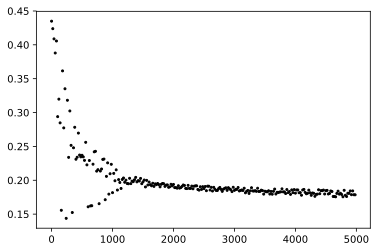
\includegraphics{sprawozdanie/output_0_9.pdf}
 % output_0_1.pdf: 382x252 px, 72dpi, 13.48x8.89 cm, bb=0 0 382 252
\end{center}

\begin{lstlisting}[language=xml]
    <HiddenLayers>
        <Layer>
            <Neuron>
                <Output>1.654327342072491e-10</Output>
                <Weights>
                    <Weight>-1.1570798721028488</Weight>
                    <Weight>23.14699099579169</Weight>
                    <Weight>17.683572379823403</Weight>
                    <Weight>-22.523697466001249</Weight>
                </Weights>
            </Neuron>
            <Neuron>
                <Output>0.9999999985678607</Output>
                <Weights>
                    <Weight>20.964295210079612</Weight>
                    <Weight>-17.939772416189577</Weight>
                    <Weight>-1.1583672675525389</Weight>
                    <Weight>20.365583524271486</Weight>
                </Weights>
            </Neuron>
        </Layer>
    </HiddenLayers>

\end{lstlisting}
\clearpage
\subsection{Bez momentum, z biasem, nauka 0.9, 5000 epok}
\begin{lstlisting}[language=bash]
$ ./perceptron -c 4 2 4 -e 5000 -l 0.9 -m 0.0 --with-bias \
  --log-learning ../data/e5000l09m00b \
  --serialize ../data/e5000l09m00b.xml
\end{lstlisting}
\begin{center}
 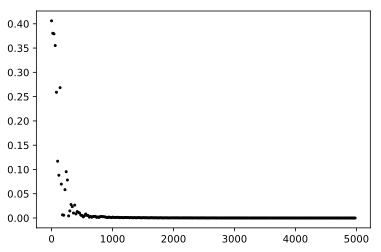
\includegraphics{sprawozdanie/output_0_11.pdf}
 % output_0_1.pdf: 382x252 px, 72dpi, 13.48x8.89 cm, bb=0 0 382 252
\end{center}
\begin{lstlisting}[language=xml]
    <HiddenLayers>
        <Layer>
            <Neuron>
                <BiasWeight>-34.644727790712956</BiasWeight>
                <Output>0.88762062849738677</Output>
                <Weights>
                    <Weight>36.717244419279439</Weight>
                    <Weight>-22.044120292292256</Weight>
                    <Weight>-86.032011522319863</Weight>
                    <Weight>36.580444905716512</Weight>
                </Weights>
            </Neuron>
            <Neuron>
                <BiasWeight>-53.204280989612798</BiasWeight>
                <Output>0.8226163509547747</Output>
            </Neuron>
        </Layer>
    </HiddenLayers>
\end{lstlisting}
\clearpage
\subsection{Bez momentum, z biasem, nauka 0.6, 5000 epok}
\begin{lstlisting}[language=bash]
$ ./perceptron -c 4 2 4 -e 5000 -l 0.6 -m 0.0 --with-bias \
  --log-learning ../data/e5000l06m00b \
  --serialize ../data/e5000l06m00b.xml
\end{lstlisting}
\begin{center}
 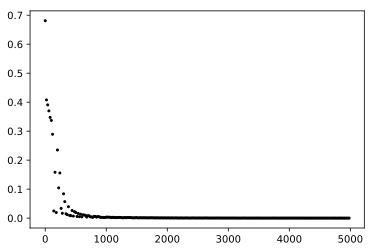
\includegraphics{sprawozdanie/output_0_13.pdf}
 % output_0_1.pdf: 382x252 px, 72dpi, 13.48x8.89 cm, bb=0 0 382 252
\end{center}
\begin{lstlisting}[language=xml]
    <HiddenLayers>
        <Layer>
            <Neuron>
                <BiasWeight>-30.092977528895702</BiasWeight>
                <Output>1.2655005212062295e-23</Output>
                <Weights>
                    <Weight>-22.637854273526603</Weight>
                    <Weight>32.052383687077615</Weight>
                    <Weight>-71.394057788154555</Weight>
                    <Weight>31.865767774502743</Weight>
                </Weights>
            </Neuron>
            <Neuron>
                <BiasWeight>-43.386898930034071</BiasWeight>
                <Output>1.1183168545617627e-55</Output>
                <Weights>
                    <Weight>-83.155401399448706</Weight>
                    <Weight>44.997837960157824</Weight>
                    <Weight>44.390776798234896</Weight>
                    <Weight>-48.874384885776045</Weight>
                </Weights>
            </Neuron>
        </Layer>
    </HiddenLayers>
\end{lstlisting}
\clearpage
\subsection{Bez momentum, z biasem, nauka 0.2, 5000 epok}
\begin{lstlisting}[language=bash]
$ ./perceptron -c 4 2 4 -e 5000 -l 0.2 -m 0.0 --with-bias \
  --log-learning ../data/e5000l02m00b \
  --serialize ../data/e5000l02m00b.xml
\end{lstlisting}
\begin{center}
 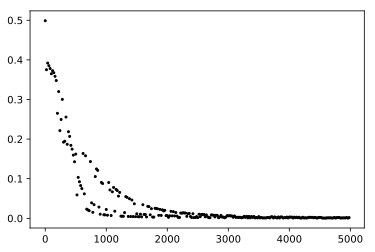
\includegraphics{sprawozdanie/output_0_15.pdf}
 % output_0_1.pdf: 382x252 px, 72dpi, 13.48x8.89 cm, bb=0 0 382 252
\end{center}
\begin{lstlisting}[language=xml]
    <HiddenLayers>
        <Layer>
            <Neuron>
                <BiasWeight>-15.545519030757312</BiasWeight>
                <Output>5.3212122090108794e-37</Output>
                <Weights>
                    <Weight>17.075943978985112</Weight>
                    <Weight>12.454494796473394</Weight>
                    <Weight>22.363802480167418</Weight>
                    <Weight>-67.989924518982221</Weight>
                </Weights>
            </Neuron>
            <Neuron>
                <BiasWeight>-29.443979969869851</BiasWeight>
                <Output>0.60905092456831877</Output>
                <Weights>
                    <Weight>31.028658960779936</Weight>
                    <Weight>-84.173329550478542</Weight>
                    <Weight>-5.1175377550280334</Weight>
                    <Weight>29.895078753162743</Weight>
                </Weights>
            </Neuron>
        </Layer>
    </HiddenLayers>
\end{lstlisting}
\clearpage
\subsection{Momentum 0.6, z biasem, nauka 0.9, 5000 epok}
\begin{lstlisting}[language=bash]
$ ./perceptron -c 4 2 4 -e 5000 -l 0.9 -m 0.6 --with-bias \
  --log-learning ../data/e5000l09m06b \
  --serialize ../data/e5000l09m06b.xml
\end{lstlisting}
\begin{center}
 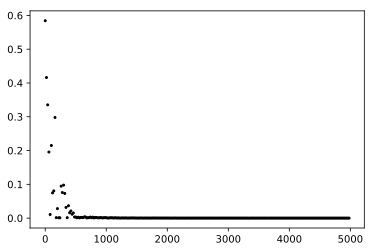
\includegraphics{sprawozdanie/output_0_17.pdf}
 % output_0_1.pdf: 382x252 px, 72dpi, 13.48x8.89 cm, bb=0 0 382 252
\end{center}
\begin{lstlisting}[language=xml]
     <HiddenLayers>
        <Layer>
            <Neuron>
                <BiasWeight>-0.42892511619098661</BiasWeight>
                <Output>0.10574171291679138</Output>
                <Weights>
                    <Weight>131.24526439214549</Weight>
                    <Weight>-44.866017715902004</Weight>
                    <Weight>-2.1360794256948386</Weight>
                    <Weight>-2.1360062774782786</Weight>
                </Weights>
            </Neuron>
            <Neuron>
                <BiasWeight>-0.35061174103949877</BiasWeight>
                <Output>0.10613838579640701</Output>
                <Weights>
                    <Weight>-38.479399308232075</Weight>
                    <Weight>128.47124462745174</Weight>
                    <Weight>-2.131816121105345</Weight>
                    <Weight>-2.1314951800557194</Weight>
                </Weights>
            </Neuron>
        </Layer>
    </HiddenLayers>
\end{lstlisting}
\clearpage
\subsection{Momentum 0.9, z biasem, nauka 0.2, 5000 epok}
\begin{lstlisting}[language=bash]
$ ./perceptron -c 4 2 4 -e 5000 -l 0.2 -m 0.9 --with-bias \
  --log-learning ../data/e5000l02m09b \
  --serialize ../data/e5000l02m09b.xml
\end{lstlisting}
\begin{center}
 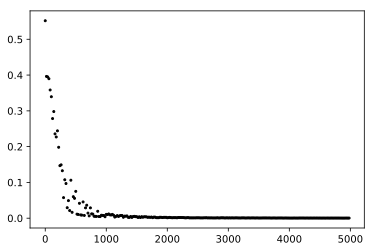
\includegraphics{sprawozdanie/output_0_19.pdf}
 % output_0_1.pdf: 382x252 px, 72dpi, 13.48x8.89 cm, bb=0 0 382 252
\end{center}
\begin{lstlisting}[language=xml]
     <HiddenLayers>
        <Layer>
            <Neuron>
                <BiasWeight>-0.42892511619098661</BiasWeight>
                <Output>0.10574171291679138</Output>
                <Weights>
                    <Weight>131.24526439214549</Weight>
                    <Weight>-44.866017715902004</Weight>
                    <Weight>-2.1360794256948386</Weight>
                    <Weight>-2.1360062774782786</Weight>
                </Weights>
            </Neuron>
            <Neuron>
                <BiasWeight>-0.35061174103949877</BiasWeight>
                <Output>0.10613838579640701</Output>
                <Weights>
                    <Weight>-38.479399308232075</Weight>
                    <Weight>128.47124462745174</Weight>
                    <Weight>-2.131816121105345</Weight>
                    <Weight>-2.1314951800557194</Weight>
                </Weights>
            </Neuron>
        </Layer>
    </HiddenLayers>
\end{lstlisting}
\clearpage
\section{Wnioski}
\subsection{Wpływ biasu na szybkość nauki}
Na podstawie przeprowadzonych obserwacji można jednoznacznie stwierdzić, że obecność dodatkowej wagi parametryzowanej stałym wejściem o wartości 1 pozwala przyspieszyć proces nauki. Spośród przeprowadzonych prób wyłącznie raz udało osiągnąć się zbieżność - przy czym błąd ma i tak relatywnie dużą wartość, co pokazują przykłady z włączoną obecnością biasu.
\subsection{Wpływ momentum}
Zastosowanie momentum pozwoliło sieci dużo szybciej dojść do powtarzalności w poprawności udzielanych odpowiedzi. Widać to bardzo dobrze na wykresach 4.5 i 4.7. Jeśli użyjemy momentum do aktualizacji wag, proces nauki staje się ``płynniejszy''. Z obserwowanych prób można by wysnuć hipotezę, że zastosowanie momentum może również pomóc w zbieżności funkcji, jednak wystarczyła jedna próba przeprowadzona dla 100000 epok aby ową hipotezę odrzucić:
\begin{lstlisting}[language=xml]
 $ ./perceptron -c 4 2 4 -m0.9 -l0.2 -e 100000 \
   --log-learning ../data/e100000l02m09
\end{lstlisting}

\begin{center}
 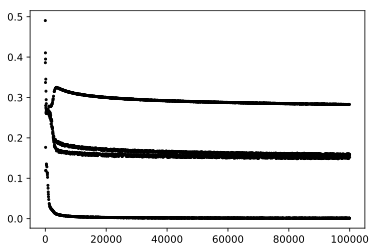
\includegraphics{sprawozdanie/output_0_21.pdf}
 % output_0_1.pdf: 382x252 px, 72dpi, 13.48x8.89 cm, bb=0 0 382 252
\end{center}

%\begin{thebibliography}{0}
  %\bibitem{l2short} T. Oetiker, H. Partl, I. Hyna, E. Schlegl.
   % \textsl{Nie za krótkie wprowadzenie do systemu \LaTeX2e}, 2007, dostępny
    %online.
%\end{thebibliography}
\end{document}
